\section{Solution}

\subsection{Analysis on the Conflicts}

\begin{frame}
	\begin{itemize}
		\item Checking correctness of partial ordering	
		\linebreak
		\begin{itemize}
			\item Formally model the graph topology mutation
			\linebreak
			\item Check if  the reordered mutation is same as the users' denoted mutation
		\end{itemize}
	\end{itemize}
\end{frame}

\begin{frame}
	\begin{itemize}
		\item Possible combinations introducing conflicts
		\linebreak
			\begin{figure}
			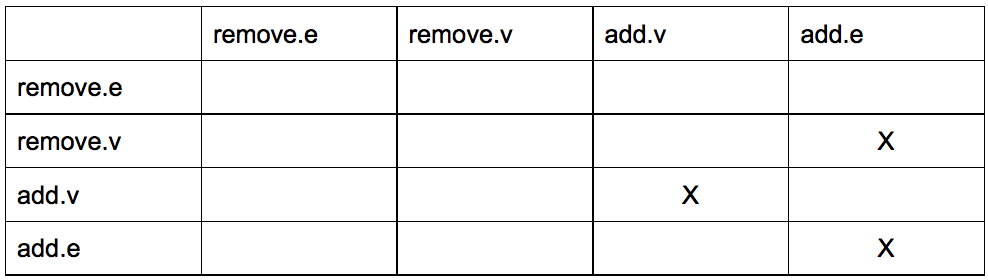
\includegraphics[width=0.8\linewidth]{Pictures/table.png}
			\caption{Combination that creates conflicts}
			\end{figure}
	\end{itemize}
\end{frame}

\begin{frame}	
		 \begin{itemize}
		      \item Refinement of the analysis
		      \linebreak
		   	  \begin{itemize}
				\item Look at the compute() of active vertices in a Superstep 
				\item Collect topolpgy mutation operations
				\item Prune the list if the operation in consideration does not fall into any categories that create conflicts
				\item Take control and data flow into consideration
				\item Formally model the graph mutation and use a proof assistant to prove the correctness of the process
		     	  \end{itemize}
		  \end{itemize}
\end{frame}


\subsection{Examples}
\begin{frame}
\begin{itemize}
  \item 
    
\end{itemize}
\end{frame}